\documentclass[pageno]{jpaper}

% \newcommand{\IWreport}{2015}

\usepackage[normalem]{ulem}

\begin{document}

\title{
Solving SAT Reading Comprehension Questions with Memory Networks}

\author{Saahil Madge\\Adviser: Professor Christiane Fellbaum}

\date{}
\maketitle

\thispagestyle{empty}
% \doublespacing
% \begin{abstract}
% This document is intended to serve as a sample you can use for independent work reports.  We provide some guidelines on content and formatting.  They are not required, but they might be helpful.
% \end{abstract}

\section{Background and Motivation}
\label{Background and Motivation}

Machine question-answering (QA) has been a popular subject in recent research.
It is a very interesting field from an academic perspective, requiring
knowledge and techniques across the areas of artificial intelligence, machine
learning, natural language processing, linguistics, and mathematics.

QA has applications to many aspects of daily life. A famous use of
question-answering techniques is in Apple's Siri program. Siri combines speech
recognition software with question-answering techniques to create a virtual
iPhone assistant. Another example is IBM's Watson, which answered questions in
many subjects and performed quite well as a contestant on the game show
\textit{Jeopardy!} A less spectacular but more commonly-used example can be seen
by typing in a simple question such as \textit{How many calories are in an
apple?} on Google. The search results provide a detailed nutritional breakdown
of an apple.

The general term QA covers a broad array of subfields. Information retrieval,
factual question-answering, reading comprehension, and inference are all part
of the greater question-answering area. QA is a rapidly evolving field, but as
the examples above indicate, recent research has focused extensively on
answering spoken questions, and factual questions.

However, the subfield of machine comprehension has not been studied nearly as
well, though it has become quite popular in the past few years. Machine
comprehension involves training programs and systems to read text and answer
questions based on the newly acquired information. In most other QA tasks, the
system has a large database of facts (knowledge base) and must interpret the
question and provide the relevant factual answer. Machine comprehension tasks,
on the other hand, require the system to parse both the informational text as
well as the question, and then provide the correct answer. As there is
possibility for error within the knowledge base, machine comprehension tasks
are some of the most difficult QA tasks.

Machine comprehension has a wide range of applications. Reading comprehension
tests are a natural choice, but fields like document retrieval also use machine
comprehension techniques. Financial firms that use news analysis to make
trading decisions heavily rely on these techniques as well. Many long-term
goals of AI such as dialogue and humanoid robots cannot be achieved without
significant advance in this area \cite{Weston2015}. Another incentive to
study machine comprehension is that new research here can be applied to drive
research in many other areas of artificial intelligence and natural language
processing.

As a consequence of machine comprehension tasks being so difficult, most
research with reading comprehension tests has focused on elementary school
level tests. The most common dataset is MCTest\cite{Richardson2013}, which we
discuss in more detail in \ref{Related Work}. This dataset is a set of passages
and reading comprehension questions created by crowdsourcing. The stories are
``carefully limited to those a young child would
understand''\cite{Richardson2013}. Another common dataset is Facebook's bAbi
dataset\cite{Weston2015}, which has a collection of short toy problems that can
be used to train machine comprehension systems. These problems could certainly
be solved by a human elementary school student. Berant et al.\cite{Berant2014}
train a system to answer questions based on a paragraph describing biological
processes, which is certainly an advanced topic, but the system is specialized
for biological tasks and not applicable as is to general reading comprehension.

In this paper we focus on SAT reading questions. The major reason is that they
are far more complex than MCTest questions and other commonly-used machine
comprehension datasets. The sentence structures, vocabulary, and topics covered
in SAT passages are all far more varied than in the other benchmarks. The
questions are much harder as well, and simply understanding the question and the
individual choices is difficult by itself. SAT questions often test underlying
themes and broad ideas rather than particular factual details (``Why'' or
``How'' questions). In contrast, MCTest questions are often of a ``Who'',
``When'', or ``What'' form, which have traditionally been easier for programs to
answer.

Another aspect that makes SAT questions so difficult is that they require
inference to answer, as opposed to just matching words or syntax. MCTest and
similar questions can mostly be answered through word-matching (discussed in
\ref{Bag-of-words}) or via syntactic matching. Word-matching means the system
will try to find which sentences in the passage have the most words in common
with the query, and use that to choose an answer. Syntactic matching is the same
principle, but aims to match syntactic structure. SAT questions, however, almost
never repeat the answer words in the question itself, and the query structure is
not correlated with passage structure. To solve these questions, our system has
to really understand the high-level concepts and information that is implied but
not directly on the surface. This is a significantly harder problem than has
been tackled before, but it is necessary to solve to continue moving forwad in
the field of machine comprehension. Essentially, by trying to answer SAT
questions we can try to solve problems that will be present in real-world
applications but have not yet been tackled by existing research.

In particular, we modify and combine two techniques: Memory Networks and
relational semantic analysis. Memory Networks were introduced by Weston et al.
in \cite{Weston2015a} and improved by Sukhbaatar et al. in
\cite{Sukhbaatar2015}. These are a particular type of neural network. We discuss
memory networks and alternatives in much greater depth in \ref{Related Work} and
\ref{Model}. Most recent machine comprehension research has focused on using
neural nets as the core system, so we use them in this paper as well. Neural
nets are a very generalizable technique and in the past decade have become very
popular. In fact, advances in neural net techniques have greatly contributed to
the recent surge in machine comprehension research.

Memory Networks require the input text and the query to be embedded in some form
for easy computation. These embedding techniques are covered in detail in
\ref{Representation Techniques}. Typically the embedding is done with
bag-of-words embedding. This embedding technique relies on the same word being
used in the answer choices as well as in the original text, which is true for
MCTest and tests of similar difficulty. However, SAT reading comprehension
passages often have very complex answer choices that rarely use the exact same
word as used in the text. As a result we have to change the way we represent and
parse the text. Instead of using \textit{one-hot} vector encoding and picking
answer choices based on how many words are in common with the query or text, we
represent the text using relational logic. Essentially we dynamically create a
``Knowledge Graph'' as we parse through the text and try to frame each question
as a query on this knowledge graph. We enhance a tensor factorization method
known as RESCAL \cite{Bader2007}\cite{Nickel2011} and use this enhanced method
to embed the text, questions, and answers. Once the embedding is done we can
train our Memory Network on the text and query to find the answer. The knowledge
graph representation is typically used for factual data that has already been
collected in entity-relation triple form. As far as we know, no previous
research in this space has tried to dynamically create a knowledge graph on
which we can answer questions.

Our goal with this research is to present a way to combine ideas that were
previously used in isolation for QA or other learning tasks into a system which
can parse and interpret a complex text, and answer difficult high-level
questions about the text. The text, questions, and techniques we use are more
ambitious than those studied in previous research. Our results should be
interpreted as merely proof-of-concept. We hope that this paper will encourage
others to tackle problems of equal or greater ambition, and drive progress in
the development of safe artificial intelligence.

\section{Technical Review}
\label{Technical Review}

In this section we review some of the techniques that are used in previous
research and in this paper.

\subsection{Embedding Techniques}
\label{Embedding Techniques}

We begin by reviewing various methods for embedding text and performing queries
on the embedded representations. \\

\subsubsection{Bag-of-words}
\label{Bag-of-words}

Bag-of-words is a type of analysis in which we treat each sentence as simply a
collection of words, without paying attention to their order or the dependencies
between individual words. If we have some vocabulary of size $V$, we can encode
each sentence as a vector of size $V$ where each vector element corresponds to
some word in the vocabulary. If the word appears in the sentence we store how
many times it appears, and if it does not appear we store it as a 0. This is
known as \textit{one-hot} vector encoding. Most designs encode each input
sentence and the query as one-hot vectors. These vectors are not used as-is, but
are first embedded into some dimension $d$. The learning algorithm is run on the
embedded vectors, and we can output a response in a specified format. Two common
methods are to return a probability vector of size $V$ where each element
represents how likely that word is to be the output, or to pick the most likely
word from that distribution and return only that word. \\

\subsubsection{word2vec}
\label{word2vec}

The \textit{word2vec} embedding technique introduced by Mikolov et al.
\cite{Mikolov2013} is perhaps the most common embedding technique used in NLP
research. It is actually an umbrella term for various methods, such as
\textit{skip-gram} or even bag-of-words embedding. The word2vec techinque
produces a vector representation of words, often with several hundred elements.
These representations can then be manipulated as vectors in the
higher-dimensional space, allowing for interesting operations on words. For
example, \textbf{vector(``king'')} - \textbf{vector(``man'')} +
\textbf{vector(``woman'')} produces a vector that is very close to
\textbf{vector(``queen'')}. The reason word2vec is able to embed so successfully
is generally thought to be the fact that the process of embedding gives
similar words a similar embedding (which is measured by cosine similarity). \\

\subsubsection{Knowledge Graph}
\label{Knowledge Graph}

A knowledge graph generally refers to a set of \textit{entity-relation triples}.
These triples take the form $\langle e_1, r, e_2 \rangle$. where $e_1$ and $e_2$
are entities and $r$ describes the relation between these two entities. Entities
and relations can be repeated across triples. The total set of triples denotes
all the knowledge in our ``Knowledge Base''.

\begin{figure}
    \centering
    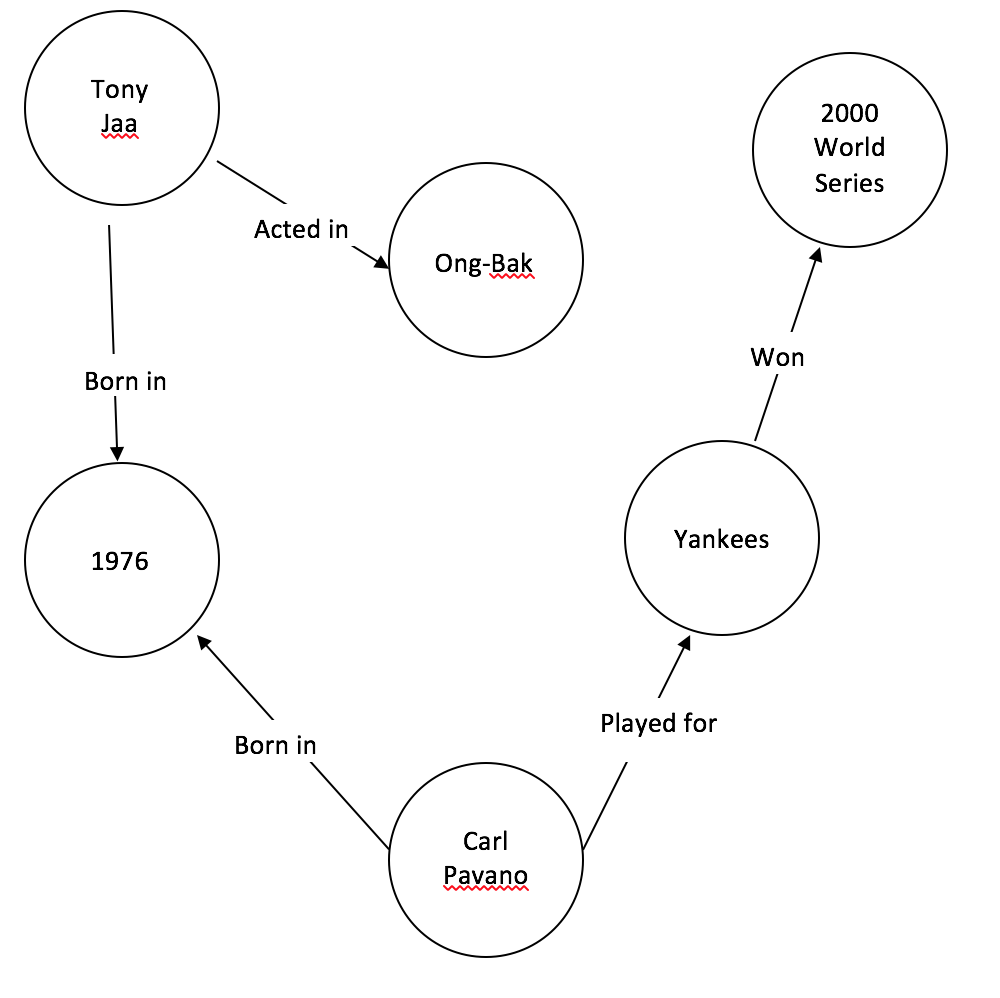
\includegraphics[width=0.7\textwidth,keepaspectratio]{figures/Example_KG.png}
    \caption{A small example knowledge graph}
    \label{Figure: KG}
\end{figure}

We can represent these triples as a directed graph, with each entity as a vertex
and the relations as edge types between them. Figure \ref{Figure: KG} shows an
example of a very small knowledge graph. Note that there is only one node per
entity. The mathematical details of our knowledge graph model can be found in
\ref{Model}.

\subsection{Neural Networks}
\label{Neural Networks}

As discussed in \ref{Background and Motivation}, recent research in machine
comprehension has extensively used neural nets (NNs) and their variants. Here we
provide a quick review of neural network design. These topics can be covered in
far more depth in \cite{Bishop1995} and \cite{Nielsen2015}.

The most basic model is known as a \textit{feed-forward} neural net. These have
several layers composed of units (nodes). There is an initial input layer, a
final output layer, and \textit{hidden layers} in the middle. A unit in layer
$l$ takes as input the output of nodes in the previous layer (or the actual
input if this is the input layer). It multiplies these by some weight matrix
$W^l$, transforms it using an activation function $g$, and sends its output to the
next layer (or as the final output if this is the output layer). Common
activation functions are the $tanh$ and $sigmoid$ functions. The sigmoid
function is defined as $\sigma (x) = \frac{1}{1+e^{-x}}$. For now we will assume
that our activation function is sigmoid.

Mathematically, we define the input to the current layer as $x^{l-1}$,
where $x^{l-1}_{ij}$ means that it is the input from unit $j$ in the previous
layer to unit $i$ in the current layer. $W^l_{ij}$ is the weight on this
connection, defined as 0 if node $i$ does not depend on node $j$. The output of
node $j$ is $\sigma ( W^l x^{l-1}_j)$. Typically the quantity $Wx^{l-1}_j$ is
known as $z_j$. We can also define bias vectors $b$ such that $z_j =
W^lx^{l-1}_j + b^l_j$. To summarize, we can write the output of some layer $l$
in vector notation as
$$o^l = \sigma(W^lx^{l-1} + b^l)$$

We can propagate this forward starting at the input layer, through the hidden
layers, and finally at our output layer. We can then train our network using the
backpropagation algorithm. We have some cost function $C$ that is a measure of
the error of our output. We find the error at the output layer, and then change
the weights at each previous layer, working backwards to the input layer. The
key to backpropagation relies on updating the weights based on their partial
derivatives with relation to $C$. In-depth derivations are provided in
\cite{Bishop1995} and \cite{Nielsen2015}.\\

\subsubsection{Recurrent Neural Networks}
\label{Recurrent Neural Networks}

Feed-forward networks are good tools, but do not have any form of state
(memory). Here we review recurrent neural networks (RNNs) which have a hidden
state $h_t$.

At step $t$ in a recurrent neural network, we have input $x_t$ and a hidden
state $h_{t-1}$. We also have weight matrices $U$ and $W$. We can define the
current state $h_t = \sigma(Ux_t + Wh_{t-1})$. We have another weight matrix $V$
for the output. The output $y_t = softmax(h_t)$, where $softmax(z_i) =
\frac{e_{z_i}}{\sum_j e^{z_j}}$. The softmax function output is a probability
distribution over the vector.

Using the softmax function has several advantages. Because it is a smooth
function, we can take its derivative, making it easier to calculate the
backpropagation equations. Additionally, most RNNs and variants use a loss
function known as cross-entropy loss. If the model output is $\hat{y}$ and the
real (target) is $y$, then cross-entropy loss is defined as $\sum_i y_i
\log(\hat{y_{i}})$. When we pair a softmax output with cross-entropy loss, the
error at the output node $i$ is simply $\hat{y_i} - y_i$. This is very
convenient because it can be calculated rapidly, so it allows for fast training
of the RNN. Training is normally a bottleneck, and by combining a robust output
function and robust loss function we get a very elegant output error. As this is
a very important result, we have included it in \ref{Derivation of Output Layer
Error}.

\section{Related Work}
\label{Related Work}

The first major research in machine comprehension was conducted by Hirschman,
et al.\cite{Hirschman1999}. Their system ``Deep Read'' takes a story and a
series of questions as input, and proposes answers by using bag-of-words
techniques with other methods such as stemming and pronoun resolution layered
on top. On a collection of remedial reading questions for grades 3-6, Deep Read
answered about 40\% of the questions correctly.

Most recent research has used the MCTest\cite{Richardson2013}, released by
Richardson, et al. at Microsoft research. There are a total of 500 passages,
each with 400 questions, created at the reading level of a young child. The
stories are fictitious, which means the answers can only be found in the story
itself. Richardson et al. also provide two baseline implementations to serve as
a benchmark. The first is a simple bag-of-words model with a sliding window. It
scores about 51\% accuracy on the MC500 questions. The second implementation
adds a distance-based scoring metric and reaches 56\% accuracy. Both
implementations score significantly higher on questions where the answer is
contained in just one sentence than on questions where the answer requires
information across multiple sentences.

Narasimhan and Barzilay\cite{Narasimhan2015} also work on the MCTest tasks.
Their main insight is to create a task-specific discourse parser to capture
specific discourse relations in the MCTest passages, while the prevailing
method had been to use generalized off-the-shelf discourse parsers. They create
three models of increasing complexity. The first assumes each question can be
answered using just one sentence, and estimates a joint probability
distribution across the question, query, and answer. The second model adds in
the joint distribution across a second sentence as well, to handle the case in
which the answer needs two sentences to answer. The third model incorporates
discourse relations between the two sentences to better understand the
relationship between information in each sentence. The relations are defined as
``Causal'', ``Temporal'', ``Explanation'', and ``Other''. Most systems have
performed the worst on these types of questions. By focusing specifically on
modeling these explanatory relations, the third model easily outscores the
other two, and the two MCTest baseline implementations, achieving almost 64\%
accuracy.

Berant et al.\cite{Berant2014} also focus on analyzing inter-sentence
relations, with application specifically to passages and questions about
biological processes. These passages generally describe a chemical reaction or
other process in which there are various starting entities which interact with
each other and form a new output. Understanding how the inputs interact and
tracing the flow of the process is crucial to answering the question. To solve
this, Berant et al. define events (or non-events) as ``triggers'', and try to
find relationships between events. The events can be thought of as nodes on a
graph, with an edge defining some relation between the two. There are eight
possible relations, including ``cause'', ``enable'', and ``prevent''. They
first create events and then predict relations between the events. The queries
are also formulated as a graph. They are categorized as dependency questions,
temporal questions, or true-false questions. This model scores almost 67\% on
the dataset, over 6\% better than the next-best model.

Weston et al.\cite{Weston2015a} introduced memory networks. These are a type of
neural network which simulate a long-term memory. We discussed in \ref{Recurrent
Neural Networks} how RNNs have a ``vanishing gradient'' problem, and are not
able to take advantage of states from more than a few steps prior. Memory
networks have a memory module which stores old memories and then updates them
given new inputs. When given a query, the memory network finds relevant
memories, then finds memories that are relevant given those memories, and so on.
Finally, it provides an answer to the query. Sukhbaatar et
al.\cite{Sukhbaatar2015} improved this model by creating a model that can be
trained end to end, while in the original design each module needed to be
trained independently. This is the model that is the basis for our design, so we
discuss it in more detail in \ref{Model}. Kumar et al.\cite{Kumar2015} create
``Dynamic Memory Networks''. Their design uses two memory modules. The semantic
memory module stores general knowledge, while the episodic memory module
iteratively finds memories relevant to the query.

\section{Data}
\label{Data}

For preliminary testing, we use both the MCTest \cite{Richardson2013} dataset as
well as the Facebook bAbi dataset \cite{Weston2015}. The MCTest baseline
algorithms provide a benchmark to test our preliminary bag-of-words
implementations against. The bAbi dataset is used to evaluate
\cite{Sukhbaatar2015}. We use the same model so our preliminary neural net
implementation is also evaluated on the bAbi dataset. However, we do not use as
many training optimizations. These comparisons are meant to be benchmark
comparisons, rather than trying to perform better.

The crux of our project relies on SAT reading comprehension tests for both
training and testing. As there are no publicly available datasets, we tried
contacting ETS to obtain a research dataset. As we have not yet heard a response,
we also collected practice SAT tests from prep books. As of now we have 8 tests
from a CollegeBoard prep book, and 11 from a Princeton Review prep book (10 full
practice tests and 1 practice PSAT test). We already owned these prep books.

Each practice test contains 3 reading sections. Each reading section has
approximately 18 comprehension questions. About 4-6 of these are from short
passages (100 words), and the remaining are from longer passages (450-500
words). There are 2 short passages and 1-2 long passages per section, each
followed by comprehension questions. Hereafter we use ``test'' to refer to just
the 3 reading sections of a test, and ``reading section'' to refer to just the
reading comprehension passages and accompanying questions of each reading
section. Math and writing sections, as well as the vocabulary questions in the
reading section, are ignored.

Our practice tests are in paper format, so we must put them in an electronic
format. Amazon Mechanical Turk was used for this task. Each test was scanned,
and we approximated that typing up one test requires an hour. We requested
Master Turkers, 2 per test, and paid \$8.00 for each task. The total expenditure
was \$304.00.

\section{Progress} Besides all of the preliminary research, the basic neural
network model has been implemented, in both 1-hop and 3-hop version, as
specified in \cite{Sukhbaatar2015}. Additionally, the programs to read in and
format data from MCTest, bAbi, and the SAT tests have been written and tested.
The tests have been scanned and the Turk tasks should be finished within a week.

The remaining steps are to create a model for dependencies within sentences and
across sentences. Two approaches look promising. The first is to use a joint
probability model as defined in \cite{Narasimhan2015} and with dependency
parsing by \cite{Chen2014}. The second is to try and create a concept map that
is updated as we parse the passage. The questions can then be answered by
looking at the concept map for a particular entity. This is similar to
\cite{Bordes2015}. Once we have that we can combine the neural net with the
parsing to train our final model.

\section{Model}
\label{Model}

Our model consists of two main parts: the semantic analysis/embedding, and the
neural network. The semantic analysis is inspired by Nickel et al.
\cite{Nickel2011} and the neural network is based on the Memory Network model
introduced by Sukhbaatar et al. \cite{Sukhbaatar2015}. Because our problem is
more complex than that tackled by these original models, we have to modify the
conceptual and mathematical basis of these models. This allows us to combine the
semantic analysis and neural network learning models.

This research presents three fundamental insights.
\begin{enumerate}

    \item We treat the input text as a knowledge base and dynamically convert it
    into a knowledge graph. We can then interpret the questions as queries on
    the graph, requiring us to find an entity or relation that represents the
    answer to the question.

    \item We use tensor decomposition to embed the knowledge graph and
    questions. Most other research has used simple bag-of-words embedding or
    word2vec embedding. However, neither of these approaches are compatible

    Specifically, we use an enhanced version of
    RESCAL\cite{Nickel2011}. RESCAL by itself is a fine model, but we make it
    more accurate by adding ``Semantically Smooth Embedding''(SSE), as proposed
    by Guo et al.\cite{Guo2015}. In their original paper they propose adding
    this type of embedding to tensor decomposition as future work, so to our
    knowledge we are the first to perform tensor decomposition with SSE.

    \item We use the embedded models as inputs to a modified version of Memory
    Networks. Given a set of embedded inputs and queries, this type of neural
    network takes advantage of ``memory'' to find new facts that are relevant
    given the current set of relevant facts, but may not be relevant solely
    based on the query.

\end{enumerate}

These techniques were first introduced in previous research. However, all of
them were applied to separate domains. Neural nets have been used for machine
comprehension on MCTest, bAbi, and questions of similar difficulty. Their
embedding model is quite simple, however (often just bag-of-words). Knowledge
graphs and tensor decomposition have traditionally been used only for relational
learning when a knowledge graph or set of triples already exists.

\subsection{Knowledge Graph Representation}
\label{Knowledge Graph Representation}
We choose to represent the input as a knowledge graph

and
the goal is to answer queries linking two entities or an entity and a relation

\subsection{Tensor Decomposition Embedding}
\label{Tensor Decomposition Embedding}
Essentially, SSE enforces geometric constraints on

\subsection{Memory Networks}
\label{Memory Networks}

\bstctlcite{bstctl:etal, bstctl:nodash, bstctl:simpurl}
\bibliographystyle{IEEEtranS}
\bibliography{final_references}

\section{Appendix}
\label{Appendix}

\subsection{Derivation of Output Layer Error}
\label{Derivation of Output Layer Error}

% When we have $n$ output nodes, our cost function is $\sum^n_i y_i
% \log(\hat{y_i})$. Consider some output

\end{document}
